%% 
%% Copyright 2007, 2008, 2009 Elsevier Ltd
%% 
%% This file is part of the 'Elsarticle Bundle'.
%% ---------------------------------------------
%% 
%% It may be distributed under the conditions of the LaTeX Project Public
%% License, either version 1.2 of this license or (at your option) any
%% later version.  The latest version of this license is in
%%    http://www.latex-project.org/lppl.txt
%% and version 1.2 or later is part of all distributions of LaTeX
%% version 1999/12/01 or later.
%% 
%% The list of all files belonging to the 'Elsarticle Bundle' is
%% given in the file `manifest.txt'.
%% 

%% Template article for Elsevier's document class `elsarticle'
%% with numbered style bibliographic references
%% SP 2008/03/01

\documentclass[preprint,12pt, a4paper]{elsarticle}

%% Use the option review to obtain double line spacing
%% \documentclass[authoryear,preprint,review,12pt]{elsarticle}

%% For including figures, graphicx.sty has been loaded in
%% elsarticle.cls. If you prefer to use the old commands
%% please give \usepackage{epsfig}

%% The amssymb package provides various useful mathematical symbols
\usepackage{amssymb}
\usepackage{hyperref}
%% The amsthm package provides extended theorem environments
%% \usepackage{amsthm}

%% The lineno packages adds line numbers. Start line numbering with
%% \begin{linenumbers}, end it with \end{linenumbers}. Or switch it on
%% for the whole article with \linenumbers.
%\usepackage{lineno}

\journal{Software Impacts}

\begin{document}

\begin{frontmatter}

%% Title, authors and addresses

%% use the tnoteref command within \title for footnotes;
%% use the tnotetext command for theassociated footnote;
%% use the fnref command within \author or \address for footnotes;
%% use the fntext command for theassociated footnote;
%% use the corref command within \author for corresponding author footnotes;
%% use the cortext command for theassociated footnote;
%% use the ead command for the email address,
%% and the form \ead[url] for the home page:
%% \title{Title\tnoteref{label1}}
%% \tnotetext[label1]{}
%% \author{Name\corref{cor1}\fnref{label2}}
%% \ead{email address}
%\ead[url]{https://re2c.org}
%% \fntext[label2]{}
%% \cortext[cor1]{}
%% \address{Address\fnref{label3}}
%% \fntext[label3]{}

\title{RE2C: a lexer generator based on lookahead-TDFA}

%% use optional labels to link authors explicitly to addresses:
%% \author[label1,label2]{}
%% \address[label1]{}
%% \address[label2]{}

\author{U. Trofimovich}
\ead{skvadrik@gmail.com}

\begin{abstract}
RE2C is a regular expression compiler:
it transforms regular expressions into finite state machines
and encodes them as programs in the target language.
At the core of RE2C is the lookahead-TDFA algorithm
that allows it to perform fast and lightweight submatch extraction.
This article describes the algorithm used in RE2C and gives an example of TDFA construction.
\end{abstract}

\begin{keyword}
Lexical analysis \sep Regular expressions \sep Finite automata

%% PACS codes here, in the form: \PACS code \sep code

%% MSC codes here, in the form: \MSC code \sep code
%% or \MSC[2008] code \sep code (2000 is the default)

\end{keyword}

\end{frontmatter}

\section{Introduction}

\noindent
Regular expression engines can be divided in two categories: run-time libraries and lexer generators.
Run-time libraries perform interpretation or just-in-time compilation of regular expressions.
They use a variety of algorithms ranging from recursive backtracking to automata, string searching, or some combination of the above.
Lexer generators, on the other hand, perform ahead-of-time compilation.
They use algorithms based on deterministic finite automata (DFA) and spend considerable time on compilation and optimization in order to emit better code.
Consequently, lexer generators usually do not support features that cannot be implemented on vanilla DFA.
One such feature is submatch extraction --- the ability to find the correspondence between parts of the regular expression and parts of the input string.
Submatch extraction is a special case of the parsing problem:
in addition to solving the recognition problem it has to find the derivation of the input string in the grammar defined by the regular expression.
Unlike full parsing, submatch extraction needs only a partial derivation.
Therefore it would be wasteful to perform full parsing,
and a more specialized algorithm is needed that has overhead proportional to submatch detalization.
For an optimizing lexer generator like RE2C \cite{RE2C} \cite{RE2Cx} it is important that the generated code is at least as fast and memory-efficient as hand-written code,
and there is zero overhead if submatch extraction is not used.

\section{Tagged DFA}

\noindent
The above requirements place tight constraints on the submatch extraction algorithm:
it should be a one-pass DFA-based algorithm that works in constant memory independent of the input length.
Such an algorithm was invented by Ville Laurikari \cite{Lau00}.
It works as follows.
First, the regular expression is converted to a nondeterministic finite automaton with tagged transitions (TNFA).
Tags are submatch markers that can be placed anywhere in the regular expression;
for example, a capturing group can be represented with a pair of tags for the opening and closing parentheses.
TNFA is in essence a nondeterministic finite state transducer that rewrites symbolic strings into tagged strings.
The most important part of Laurikari algorithm is TNFA determinization.
Its basic principle is the same as in the powerset construction that converts NFA to DFA:
the NFA is simulated on all possible input strings, maintaining a set of states at each step.
If the current state-set is new, it becomes a new DFA state, otherwise it is mapped to an existing DFA state.
In the Laurikari algorithm state-sets are augmented with tag information:
each TNFA substate has an associated vector of registers that store tag values,
so that the whole state-set is a matrix indexed by TNFA states and tags.
Registers are needed because different substates are reached by different TNFA paths,
and the tags along one path may disagree with tags along another path.
If a tag is updated on a TNFA path, its value is stored into a new register.
The augmented state-sets cannot be mapped in the same way as ordinary DFA states,
because a pair of state-sets may have identical TNFA substates, but different registers.
The key insight is that mapping of such state-sets is still possible if there is a bijection between their registers:
the bijective transformation can be encoded in the form of register reordering operations on TDFA transitions.
After determinization all the information in TDFA state-sets is erased,
and the resulting TDFA is like ordinary DFA extended with a fixed number of registers
and operations on transitions that update and reorder tag values stored in registers.
Algorithms like minimization are applicable to TDFA,
but they need to differentiate between transitions with different register operations.

\section{Lookahead TDFA}

\begin{figure}[t!]
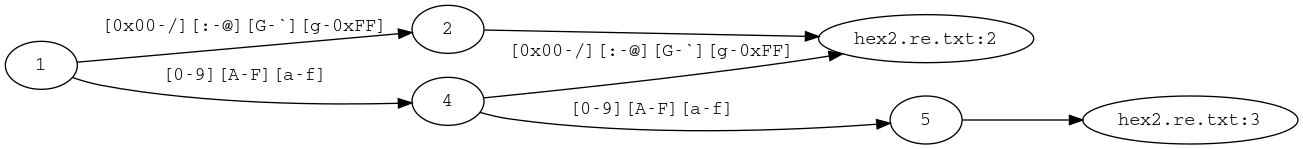
\includegraphics[width=\linewidth]{example.pdf}
%\vspace{-1em}
\caption{
Lookahead-TDFA construction for regular expression $a^* \, t_1 (t_2 \, b)^* c \;$ with tags $t_1$ and $t_2$
that matches strings $a \dots a b \dots b c$ (tag $t_1$ marks the boundary between $a$s and $b$s, and tag $t_2$ marks the last $b$).
Top: TNFA ($\epsilon/\epsilon$ labels are omitted, and negative tags indicate no-match).
Middle: lookahead-TDFA under construction with state-sets, register matrices and lookahead tags
($p$ is the current position, and $\varnothing$ is no-match).
Bottom left: lookahead-TDFA after construction.
Bottom right: lookahead-TDFA after optimization (the number of registers is minimized and some register operations are removed).
}\label{fig:example}
\end{figure}

\noindent
One improvement to Laurikari algorithm that allows to greatly reduce the number of register operations is the use of the lookahead symbol \cite{Tro17}.
The idea is to delay the application of register operations until the lookahead symbol is known,
and attach the operations to the outgoing transition on that symbol instead of the preceding incoming transition.
The insight is that some of TNFA paths that have reached the current TDFA state are canceled after the application of lookahead symbol,
and all register operations associated with these paths can be canceled as well.
In other words, delaying for one step allows one to split register operations on the lookahead symbol,
and instead of doing all of them, do only the relevant part.
This requires a modification to the underlying TDFA state-sets:
in addition to registers, each substate needs to have an associated list of lookahead tags.
The additional information is erased after determinization,
and the resulting lookahead-TDFA is faster than ordinary TDFA and better suited for further transformations like minimization and register allocation.
On the whole, this idea is similar to the improvement of LALR parsers over LR parsers:
the use of lookahead information in states greatly reduces the number of conflicts
(for TDFA a conflict is not an error, but it means extra registers and register operations).
An example of lookahead-TDFA construction can be seen on figure \ref{fig:example}.


\section{Ambiguity resolution}

\noindent
One of the challenges that makes parsing harder than recognition is ambiguity:
there may be several ways to parse the input string.
Which way to prefer is usually defined by a disambiguation policy.
TDFA algorithm can be parameterized over different policies;
for example, RE2C supports both the Perl leftmost-greedy policy and the POSIX longest-match policy \cite{BorTro19}.
Disambiguation happens at the time of determinization (in $\epsilon$-closure construction),
and the resulting TDFA does not perform any disambiguation at run-time: ambiguity-resolving decisions are embedded into its structure.

\section{Impact}

\noindent
RE2C is a lexer generator of choice for projects that need \emph{fast} lexical analyzers.
It has a flexible user interface that allows one to customize the generated code for a particular environment and input model.
Fast and lightweight submatch extraction is yet another feature that makes RE2C a good alternative to other lexer generators.
Notable projects that use RE2C are the following:

\begin{itemize}
\item Ninja, a build system with a focus on speed. \cite{Ninja}
    Ninja is used in a great number of open-source projects,
    and it is a necessary building block in many operating systems and platforms.

\item PHP, a popular general-purpose scripting language. \cite{PHP}

\item BRL-CAD, a constructive solid geometry solid modeling computer-aided design system. \cite{BRLCAD}

\item STEPCode, an implementation of ISO 10303 standard. \cite{STEPCode}

\item Apache SpamAssassin, a program for e-mail spam filtering. \cite{SpamAssassin}

\item Yasm, the Modular Assembler Project. \cite{Yasm}

\item Wake, the SiFive build tool. \cite{Wake}
\end{itemize}

\noindent
RE2C has a permissive license, which allows it to be used in proprietary software as well.
The project has been ported to many operating systems;
according to Repology \cite{Repology}, it is packaged in more than 60 distributions.
Besides being a useful practical tool, RE2C is a research playground for the development of new algorithms in the field of automata and formal languages.

\section{Conclusion and future work}

\noindent
Submatch extraction algorithm implemented in RE2C
is both an important theoretical development and a useful practical improvement.
It allows one to program lexical analyzers capable of submatch extraction
without resorting to manual post-processing or the use of string-searching functions.
The overhead on submatch extraction is proportional to submatch detalization:
there is zero overhead if no submatch information is needed,
and even for large submatch-heavy regular expressions like RFC-compliant URI and HTTP parsers the overhead is modest
(about 1.25x compared to simple recognition on DFA \cite{Tro17}).
%
Future work may relate TDFA to other parsing automata, such as DSST \cite{Gra15} and sta-DFA \cite{Cho18},
and investigate the possibility of using tagged counter automata for counted repetition \cite{Bec09}.


\section*{Acknowledgments}
\label{}
\noindent
I want to thank my parents Vladimir and Elina,
my friend and fellow researcher Angelo Borsotti,
my school math teachers Tatyana Leonidovna and Demian Vladimirovich,
and, most of all, Sergei.


\begin{thebibliography}{00}

\bibitem{RE2C}
    RE2C, a lexer generator for C, C++ and Go.
    Website: \url{https://re2c.org},
    source code: \url{https://github.com/skvadrik/re2c}.

\bibitem{RE2Cx}
    Peter Bumbulis,
    Donald D. Cowan,
    \textit{RE2C: A more versatile scanner generator},
    ACM Letters on Programming Languages and Systems (LOPLAS),
    vol. 2, 1-4,
    pp. 70-84,
    1993.

\bibitem{Lau00}
    Ville Laurikari,
    \textit{NFAs with tagged transitions, their conversion to deterministic automata and application to regular expressions},
    Proceedings Seventh International Symposium on String Processing and Information Retrieval, 2000. SPIRE 2000,
    pp. 181-187,
    URL: \url{http://laurikari.net/ville/spire2000-tnfa.pdf}.

\bibitem{Tro17}
    Ulya Trofimovich,
    \textit{Tagged Deterministic Finite Automata with Lookahead},
    arXiv:1907.08837 [cs.FL],
    2017.

\bibitem{BorTro19}
    Angelo Borsotti, Ulya Trofimovich,
    \textit{Efficient POSIX Submatch Extraction on NFA},
    preprint, 2019,
    URL: \url{https://re2c.org/2019_borsotti_trofimovich_efficient_posix_submatch_extraction_on_nfa.pdf}.

\bibitem{Ninja}
    Ninja build system,
    URL: \url{https://ninja-build.org},
    build files that use RE2C: \url{https://ninja-build.org/build.ninja.html}.

\bibitem{PHP}
    PHP Internals Book,
    chapter \textit{Building PHP},
    URL: \url{http://www.phpinternalsbook.com/php7/build_system/building_php.html}.

\bibitem{BRLCAD}
    BRL-CAD: Tools,
    URL: \url{http://sourceforge.net/p/brlcad/code/HEAD/tree/brlcad/trunk/misc/tools/re2c}.

\bibitem{STEPCode}
    STEPCode: Build Process,
    URL: \url{https://stepcode.github.io/docs/build_process}.

\bibitem{SpamAssassin}
    SpamAssassin (sa-compile),
    URL: \url{https://spamassassin.apache.org/full/3.2.x/doc/sa-compile.html}.

\bibitem{Yasm}
    Yasm,
    URL: \url{https://yasm.tortall.net}.

\bibitem{Wake}
    Wake,
    URL: \url{https://github.com/sifive/wake}.

\bibitem{Repology}
    Repology: RE2C information
    URL: \url{https://repology.org/project/re2c/information}.

\bibitem{Gra15}
    Niels Bj{\o}rn Bugge Grathwohl,
    \textit{Parsing with Regular Expressions \& Extensions to Kleene Algebra},
    DIKU, University of Copenhagen,
    2015.

\bibitem{Cho18}
    Mohammad Imran Chowdhury,
    \textit{staDFA: An Efficient Subexpression Matching Method},
    Master thesis,
    Florida State University,
    2018.

\bibitem{Bec09}
    Michela Becchi,
    \textit{Data structures, algorithms and architectures for efficient regular expression evaluation},
    Washington University In St. Louis, School of Engineering and Applied Science,
    2009.

\end{thebibliography}

\vfill\null
\clearpage

\section*{Current code version}
\label{}

\begin{table}[!h]
\begin{tabular}{|l|p{5.7cm}|p{7.3cm}|}
%\begin{tabular}{|l|p{6.5cm}|p{6.5cm}|}
\hline
\textbf{Nr.} & \textbf{Code metadata description} & \textbf{Please fill in this column} \\
\hline
C1 & Current code version & 2.0 \\
\hline
C2 & Permanent link to code/repository used for this code version &
    \textit{https://github.com/skvadrik/re2c} \\
\hline
C3  & Permanent link to Reproducible Capsule &
    \textit{https://codeocean.com/capsule/7270e8e2-5b1b-4ee4-941e-6269cf09d542/} \\
\hline
C4 & Legal Code License   & Public domain \\
\hline
C5 & Code versioning system used & Git \\
\hline
C6 & Software code languages, tools, and services used & C++, Bison, RE2C (self-hosting) \\
\hline
C7 & Compilation requirements, operating environments \& dependencies &
    OS: Linux, BSD, Nix/Guix, GNU Hurd, OS X, Windows.
    Dependencies: C++ compiler, Bash, CMake or Autotools, optional Bison and Docutils. \\
\hline
C8 & Link to developer documentation/manual & \textit{https://re2c.org} \\
\hline
C9 & Support email for questions & \textit{re2c-general@lists.sourceforge.net} \\
\hline
\end{tabular}
\caption{Code metadata (mandatory)}
\label{} 
\end{table}

\end{document}
\endinput
